\section{Caravaggio}\label{caravaggio}


\begin{figure}
\centering
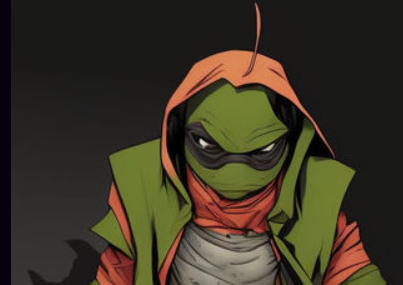
\includegraphics{Screenshot_2023-10-03_204548.png}
\end{figure}

\subsection{Descrizione Generale}\label{descrizione-generale}



Caravaggio è un monaco turtlefolk guerriero. La sua pelle verde scura e
il robusto guscio marrone lo distinguono tra gli altri della sua razza.
Caravaggio è noto per la sua lealtà, il suo coraggio e la sua
determinazione.

\begin{quote}
Citazione {[}location{]}
\end{quote}

\subsection{Biografia}\label{biografia}


Caravaggio è stato adottato da Splinter, un monaco mausefolk, insieme ai
suoi quattro fratelli. Splinter li ha cresciuti e addestrati alle arti
marziali, insegnando loro l'importanza della disciplina e della
protezione degli altri. Durante un viaggio in nave, un tremendo
naufragio ha separato Caravaggio dalla sua famiglia. Ha passato anni a
cercarla, senza mai darsi per vinto, ma non l'ha mai trovata.

\subsection{Carriera}\label{carriera}


Caravaggio ha trovato una nuova casa nelle terre di Valtara, dove ha
messo le sue abilità da combattente a servizio della gilda dei
Protettori. La sua esperienza in combattimento lo ha reso un membro
prezioso dell'organizzazione, impegnato a proteggere la regione dagli
innumerevoli pericoli che la minacciano. Il suo impegno nella gilda è
stato fonte di grande orgoglio, e ha dimostrato di essere un leader
calmo e risoluto quando è necessario.

\subsection{Personalità}\label{personalituxe0}


Caravaggio è noto per la sua lealtà e il suo coraggio. È determinato a
proteggere gli altri dopo aver perso la sua famiglia nel naufragio. Il
principale obiettivo di Caravaggio è riunirsi con i suoi fratelli e con
il suo mentore Splinter. Nel frattempo, si impegna a proteggere Valtara
e le persone che la abitano dai molteplici pericoli che la circondano.
La ricerca dei suoi fratelli è un impegno personale che lo guida in ogni
azione che intraprende.

